\section{Anàlisis i preprocessat de dades}

\subsection{Preprocessat inicial}
Una vegada importem el dataset, es pot veure que hi ha bastantes cel·les buides i altres amb el string \texttt{`NaNN'}. Per solucionar aquesta inconsistència, s'han reemplaçat tots aquests valors per \texttt{pd.NA}.

Per altra banda, s'ha declarat el tipus de cada variable correctament (com a numèriques o com a categòriques) seguint la informació que es proporciona en el metadata file (que es pot trobar en \cite{misc_cirrhosis_patient_survival_prediction_878}).

A més, com que la variable ID no és res més que l'identificador dels pacients, i no serà necessari pel nostre estudi, s'ha decidit eliminar del dataset per no haver d'eliminar-la manualment a cada procés. És a dir, entrenar un model de predicció tenint en compte l'ID del pacient no té cap sentit i només pot portar a overfitting (si troba patrons entre la variable objectiu i la variable ID). A més, a l'hora de fer gràfics no és una variable que aporti cap informació, ja que és categòrica i amb tantes classes úniques com files hi ha al dataset, de manera no es podrien interpretar els plots de cap manera.

Addicionalment, per una millor comprensió de certes variables, s'ha decidit reanomenar els seus valors, tenint en compte el metadata file, de la següent manera:
\begin{itemize}
	\item \textbf{Variable Status:}
	\begin{itemize}
		\item \textbf{`C'} $\rightarrow$ `Alive'.
		\item \textbf{`CL'} $\rightarrow$ `Liver Transplant'.
		\item \textbf{`D'} $\rightarrow$ `Dead'.
	\end{itemize}
	
	\item \textbf{Variable Edema:}
	\begin{itemize}
		\item \textbf{`N'} $\rightarrow$ `NoEdema'.
		\item \textbf{`S'} $\rightarrow$ `EdemaResolved'.
		\item \textbf{`Y'} $\rightarrow$ `EdemaPersistent'.
	\end{itemize}
	
	\item \textbf{Variable Drug:}
	\begin{itemize}
		\item \textbf{`D-penicillamine'} $\rightarrow$ 1.
		\item \textbf{`Placebo'} $\rightarrow$ 0.
	\end{itemize}
	
	\item \textbf{Variables Ascites, Hepatomegaly i Spiders:}
	\begin{itemize}
		\item \textbf{`Y'} $\rightarrow$ 1.
		\item \textbf{`N'} $\rightarrow$ 0.
	\end{itemize}
	
	
\end{itemize}

Una vegada realitzats aquests canvis, es pot començar a treballar amb el dataset correctament.

\subsection{Anàlisis estadístic de les variables i estudi de balanceig de classes}
El primer que s'ha fet per entendre el dataset i poder treballar amb ell és realitzar un anàlisis estadístic de cada una de les variables que el formen. A més, per les variables numèriques podem analitzar la distribució que segueixen mitjançant un histograma, mentre que per les categòriques podem realitzar countplots per veure la distribució entre les seves classes i com de balancejades estan.

\subsubsection{Variables numèriques}
En les taules \ref{tab:num-stats-1} i \ref{tab:num-stats-2} es poden veure estadístiques sobre totes les variables numèriques del dataset (obtingudes mitjançant la comanda \texttt{data.describe()} de la llibreria \texttt{pandas}).

% Table 1
\begin{table}[H]
\centering
\begin{tabular}{lrrrrrr}
\hline
\textbf{Statistic} & \textbf{N\_Days} & \textbf{Age} & \textbf{Bilirubin} & \textbf{Cholesterol} & \textbf{Albumin} & \textbf{Copper} \\ 
\hline
count & 418.0 & 418.0 & 418.000000 & 284.0 & 418.000000 & 310.0 \\ 
mean & 1917.782297 & 18533.351675 & 3.220813 & 369.510563 & 3.497440 & 97.648387 \\ 
std & 1104.672992 & 3815.845055 & 4.407506 & 231.944545 & 0.424972 & 85.61392 \\ 
min & 41.0 & 9598.0 & 0.300000 & 120.0 & 1.960000 & 4.0 \\ 
25\% & 1092.75 & 15644.5 & 0.800000 & 249.5 & 3.242500 & 41.25 \\ 
50\% & 1730.0 & 18628.0 & 1.400000 & 309.5 & 3.530000 & 73.0 \\ 
75\% & 2613.5 & 21272.5 & 3.400000 & 400.0 & 3.770000 & 123.0 \\ 
max & 4795.0 & 28650.0 & 28.000000 & 1775.0 & 4.640000 & 588.0 \\
\hline
\end{tabular}
\caption{Estadístiques de les variables numèriques.}
\label{tab:num-stats-1}
\end{table}

% Table 2
\begin{table}[H]
\centering
\begin{tabular}{lrrrrrr}
\hline
\textbf{Statistic} & \textbf{Alk\_Phos} & \textbf{SGOT} & \textbf{Tryglicerides} & \textbf{Platelets} & \textbf{Prothrombin} \\ 
\hline
count & 312.000000 & 312.000000 & 282.0 & 407.0 & 416.000000 \\ 
mean & 1982.655769 & 122.556346 & 124.702128 & 257.02457 & 10.731731 \\ 
std & 2140.388824 & 56.699525 & 65.148639 & 98.325585 & 1.022000 \\ 
min & 289.000000 & 26.350000 & 33.0 & 62.0 & 9.000000 \\ 
25\% & 871.500000 & 80.600000 & 84.25 & 188.5 & 10.000000 \\ 
50\% & 1259.000000 & 114.700000 & 108.0 & 251.0 & 10.600000 \\ 
75\% & 1980.000000 & 151.900000 & 151.0 & 318.0 & 11.100000 \\ 
max & 13862.400000 & 457.250000 & 598.0 & 721.0 & 18.000000 \\
\hline
\end{tabular}
\caption{Estadístiques de les variables numèriques.}
\label{tab:num-stats-2}
\end{table}


Addicionalment, en les figures \ref{fig:num-histograms-1} i \ref{fig:num-histograms-2} es poden veure les histogrames de cada una de les variables numèriques, on es veu la distribució de les seves dades ignorant els valors faltants (missings).

\begin{figure}[H]
    \centering
    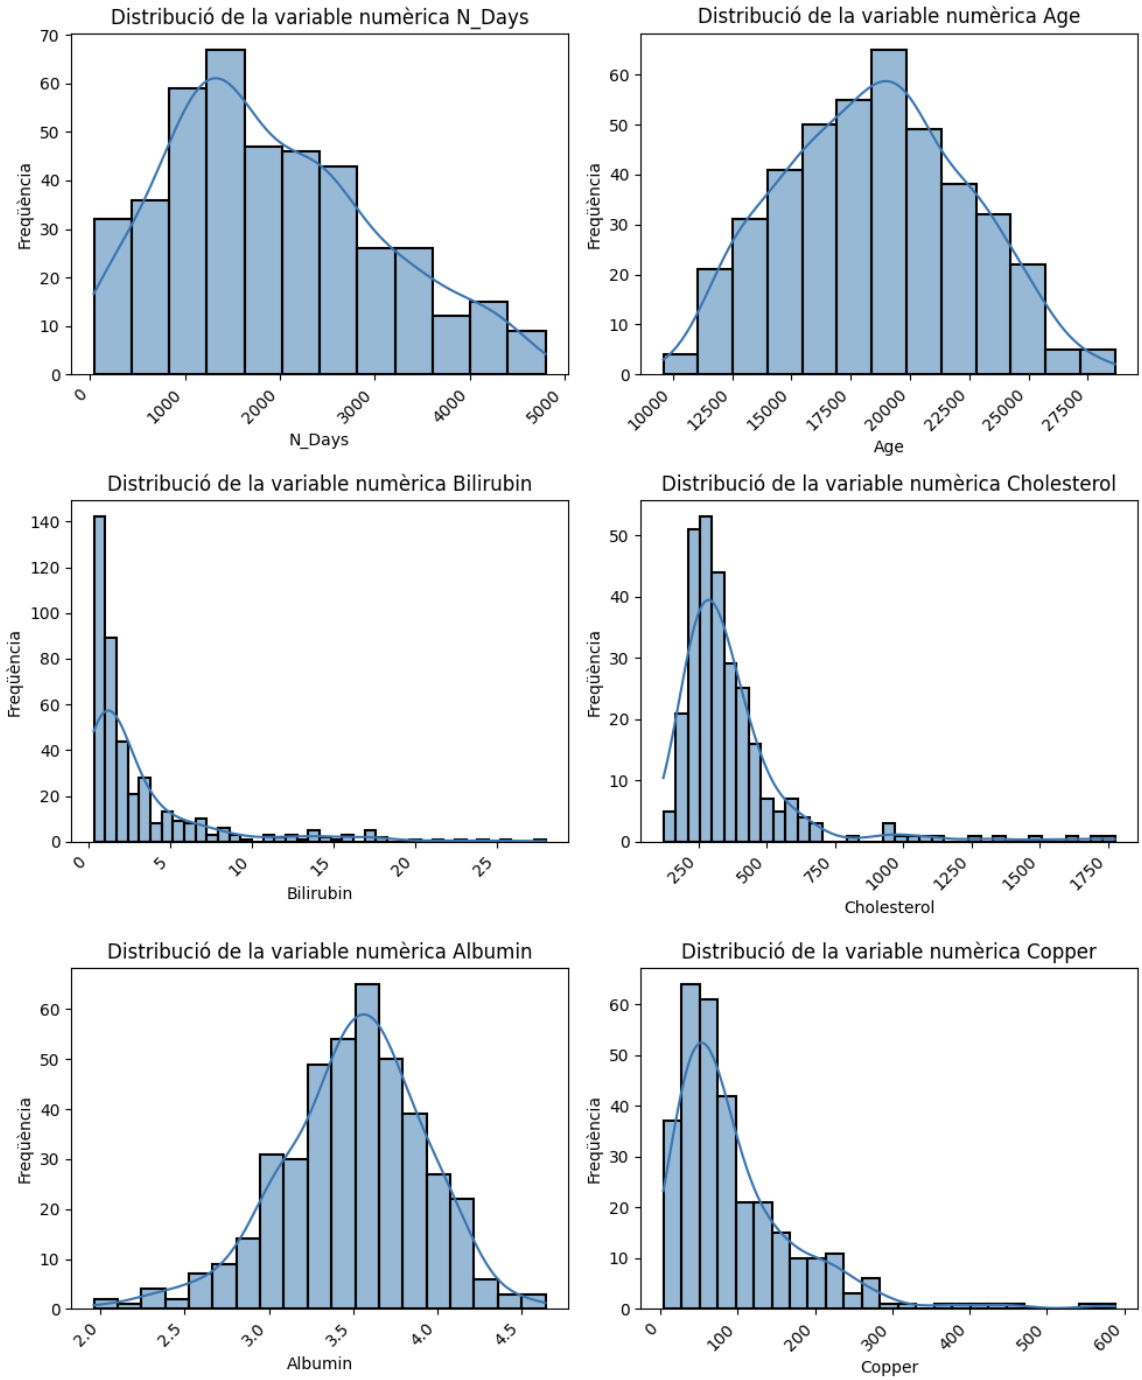
\includegraphics[width=\linewidth]{img/num-histograms-1.png}
    \caption{Histogrames de variables numèriques del datset.}
    \label{fig:num-histograms-1}
\end{figure}
\begin{figure}[H]
    \centering
    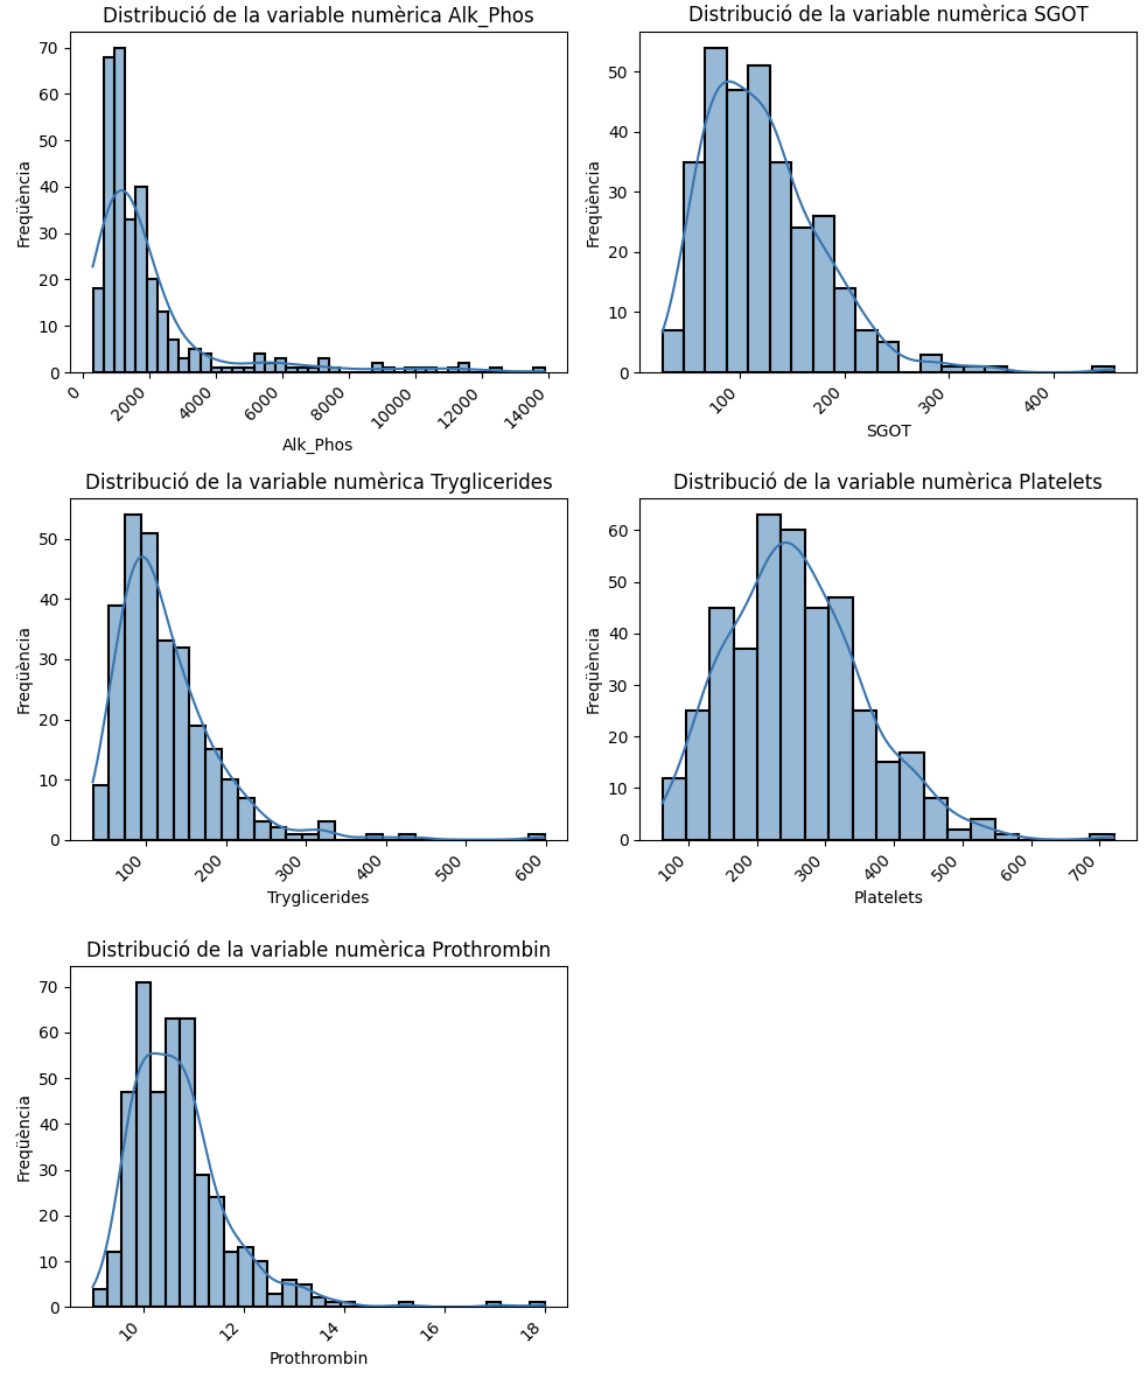
\includegraphics[width=\linewidth]{img/num-histograms-2.png}
    \caption{Histogrames de variables numèriques del datset.}
    \label{fig:num-histograms-2}
\end{figure}

\subsubsection{Variables categòriques}
En la taula \ref{tab:cat-stats-1} podem veure altres estadístiques per les variables categòriques del dataset (obtingudes mitjançant la mateixa comanda, però amb el paràmetre \texttt{include=`category'}).

\begin{table}[H]
\centering
\begin{tabular}{lrrrrrrrr}
\hline
\textbf{} & \textbf{Status} & \textbf{Drug} & \textbf{Sex} & \textbf{Ascites} & \textbf{Hepatomegaly} & \textbf{Spiders} & \textbf{Edema} & \textbf{Stage} \\ 
\hline
count & 418 & 312 & 418 & 312 & 312 & 312 & 418 & 412.0 \\ 
unique & 3 & 2 & 2 & 2 & 2 & 2 & 3 & 4.0 \\ 
top & Alive & 1 & F & 0 & 1 & 0 & NoEdema & 3.0 \\ 
freq & 232 & 158 & 374 & 288 & 160 & 222 & 354 & 155.0 \\ 
\hline
\end{tabular}
\caption{Categorical data summary of the study.}
\label{tab:cat-stats-1}
\end{table}

A més, en les figures \ref{fig:cat-countplots-1} i \ref{fig:cat-countplots-2} es poden veure els countplots de cada una de les variables categòriques, on es veu la quantitat de mostres que hi ha per cada classe de la variable, evitant els valors faltants (missings).

\begin{figure}[H]
    \centering
    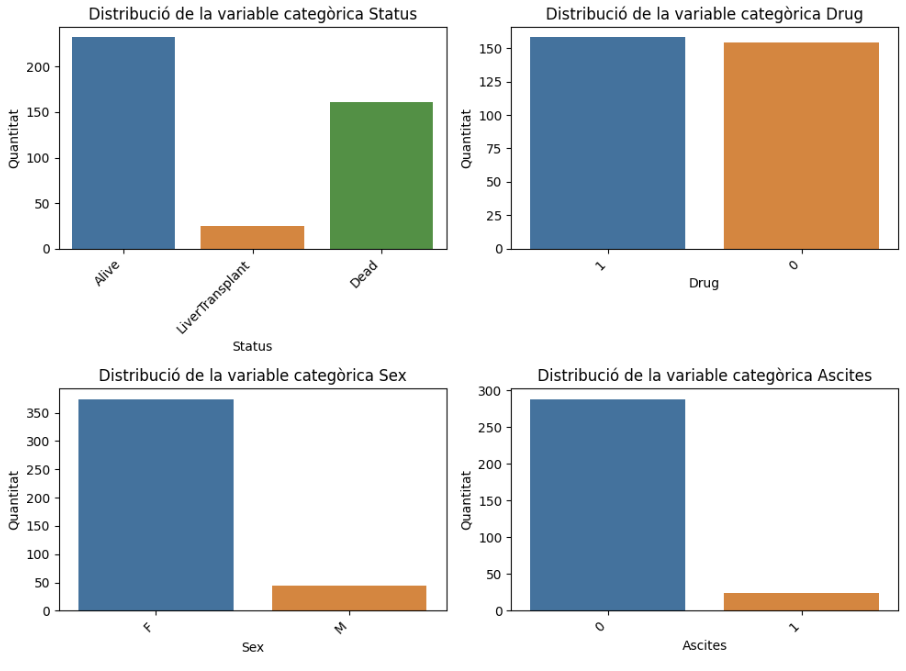
\includegraphics[width=\linewidth]{img/cat-countplots-1.png}
    \caption{Countplots de variables categòriques del datset.}
    \label{fig:cat-countplots-1}
\end{figure}
\begin{figure}[H]
    \centering
    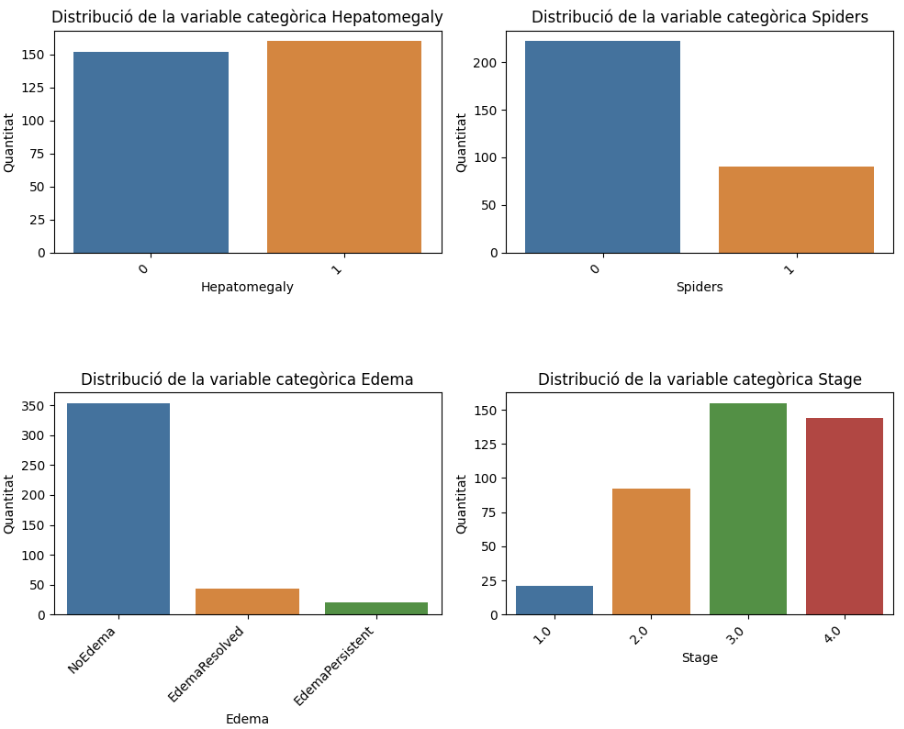
\includegraphics[width=\linewidth]{img/cat-countplots-2.png}
    \caption{Countplots de variables categòriques del datset.}
    \label{fig:cat-countplots-2}
\end{figure}

Es pot veure que les variables \textit{Status} (la variable que determinarem com a \textit{target} més endavant), \textit{Sex}, \textit{Ascites}, \textit{Spiders}, \textit{Edema} i \textit{Stage} pateixen un clar desbalanceig de classes. Això s'haurà de tenir molt en compte a l'hora de 

\subsection{Missings}

\subsection{Outliers}

\subsection{Recodificació de variables}

\subsection{Particionat del dataset}
%A partir d’aquest punt, no useu la partici ́o de validaci ́o (si heu decidit fer servir la partici ́o de validaci ́o) fins l’entrenament de models. La partici ́o de test no la podeu fer servir fins l’avaluaci ́o del model final. 1 Taula (mida de les particions). 
% –Si imputeu missings heu de particionar abans de la imputaci ́o.
%–Si feu servir un m`etode de balanceig heu de particionar abans de balancejar les classes